\documentclass{beamer}
\usetheme{Berlin}
\usecolortheme{dolphin}

\usepackage[T1]{polski}
\usepackage[polish]{babel}
\usepackage[utf8]{inputenc}
\usepackage[T1]{fontenc}
\usepackage[mediumspace,mediumqspace,Grey,squaren]{SIunits}
\usepackage{graphicx}
\usepackage{hyperref}

%\addbibresource{bibliography.bib}

\graphicspath{ {./images/} }

\begin{document}
\title{Seminarium dyplomowe magisterskie}   
\author{Jakub Postępski} 
\date{11 października 2018} 

\frame{\titlepage} 



\section{O mnie}
\begin{frame}{Zainteresowania}
\begin{itemize}
\item{Narciarstwo}
\item{Żeglarstwo}
\item{Polityka}
\item{Motoryzacja}
\end{itemize}
\end{frame}

\begin{frame}{Wykształcenie}
\begin{itemize}
\item Liceum Ogólnokształcące Jana III Sobieskiego w Lublinie
\item Wydział Elektroniki i Technik Informacyjnych: inżynier informatyk
\item W trakcie: studia magisterskie na kierunku Automatyka i~Robotyka
\end{itemize}

\begin{itemize}
	\item Członek Koła Naukowego Robotyki "Bionik"
\end{itemize}
\end{frame}

\begin{frame}{Zainteresowania naukowe}
\begin{itemize}
\item Zadania manipulacji robotów
\item Projektowanie elektroniki
\item Inżynieria biomedyczna (szczególnie BCI)
\item Programowanie funkcyjne
\end{itemize}
\end{frame}

\section{Zarys pracy magisterskiej}
\begin{frame}{Sterowanie ramieniem robota w obliczu chwytania przedmiotów}
Celem pracy jest znalezienie algorytmu kompensującego wpływ sił zewnętrznych (grawitacji) na obiekt chwytany przez robota. Praca magisterska pod kierownictwem dra inż. Tomasza Winiarskiego.


\begin{itemize}
\item Sterowanie siłowe
\item Manipulator posiada wbudowany algorytm kompensacji grawitacji dla ramienia  
\item Nieznany model chwytanego obiektu
\item Obiekt chwytany przez robota może zmieniać się w czasie
\end{itemize}
\end{frame}
\begin{frame}{Środowisko badawcze}

\begin{figure}[h]
	\centering
	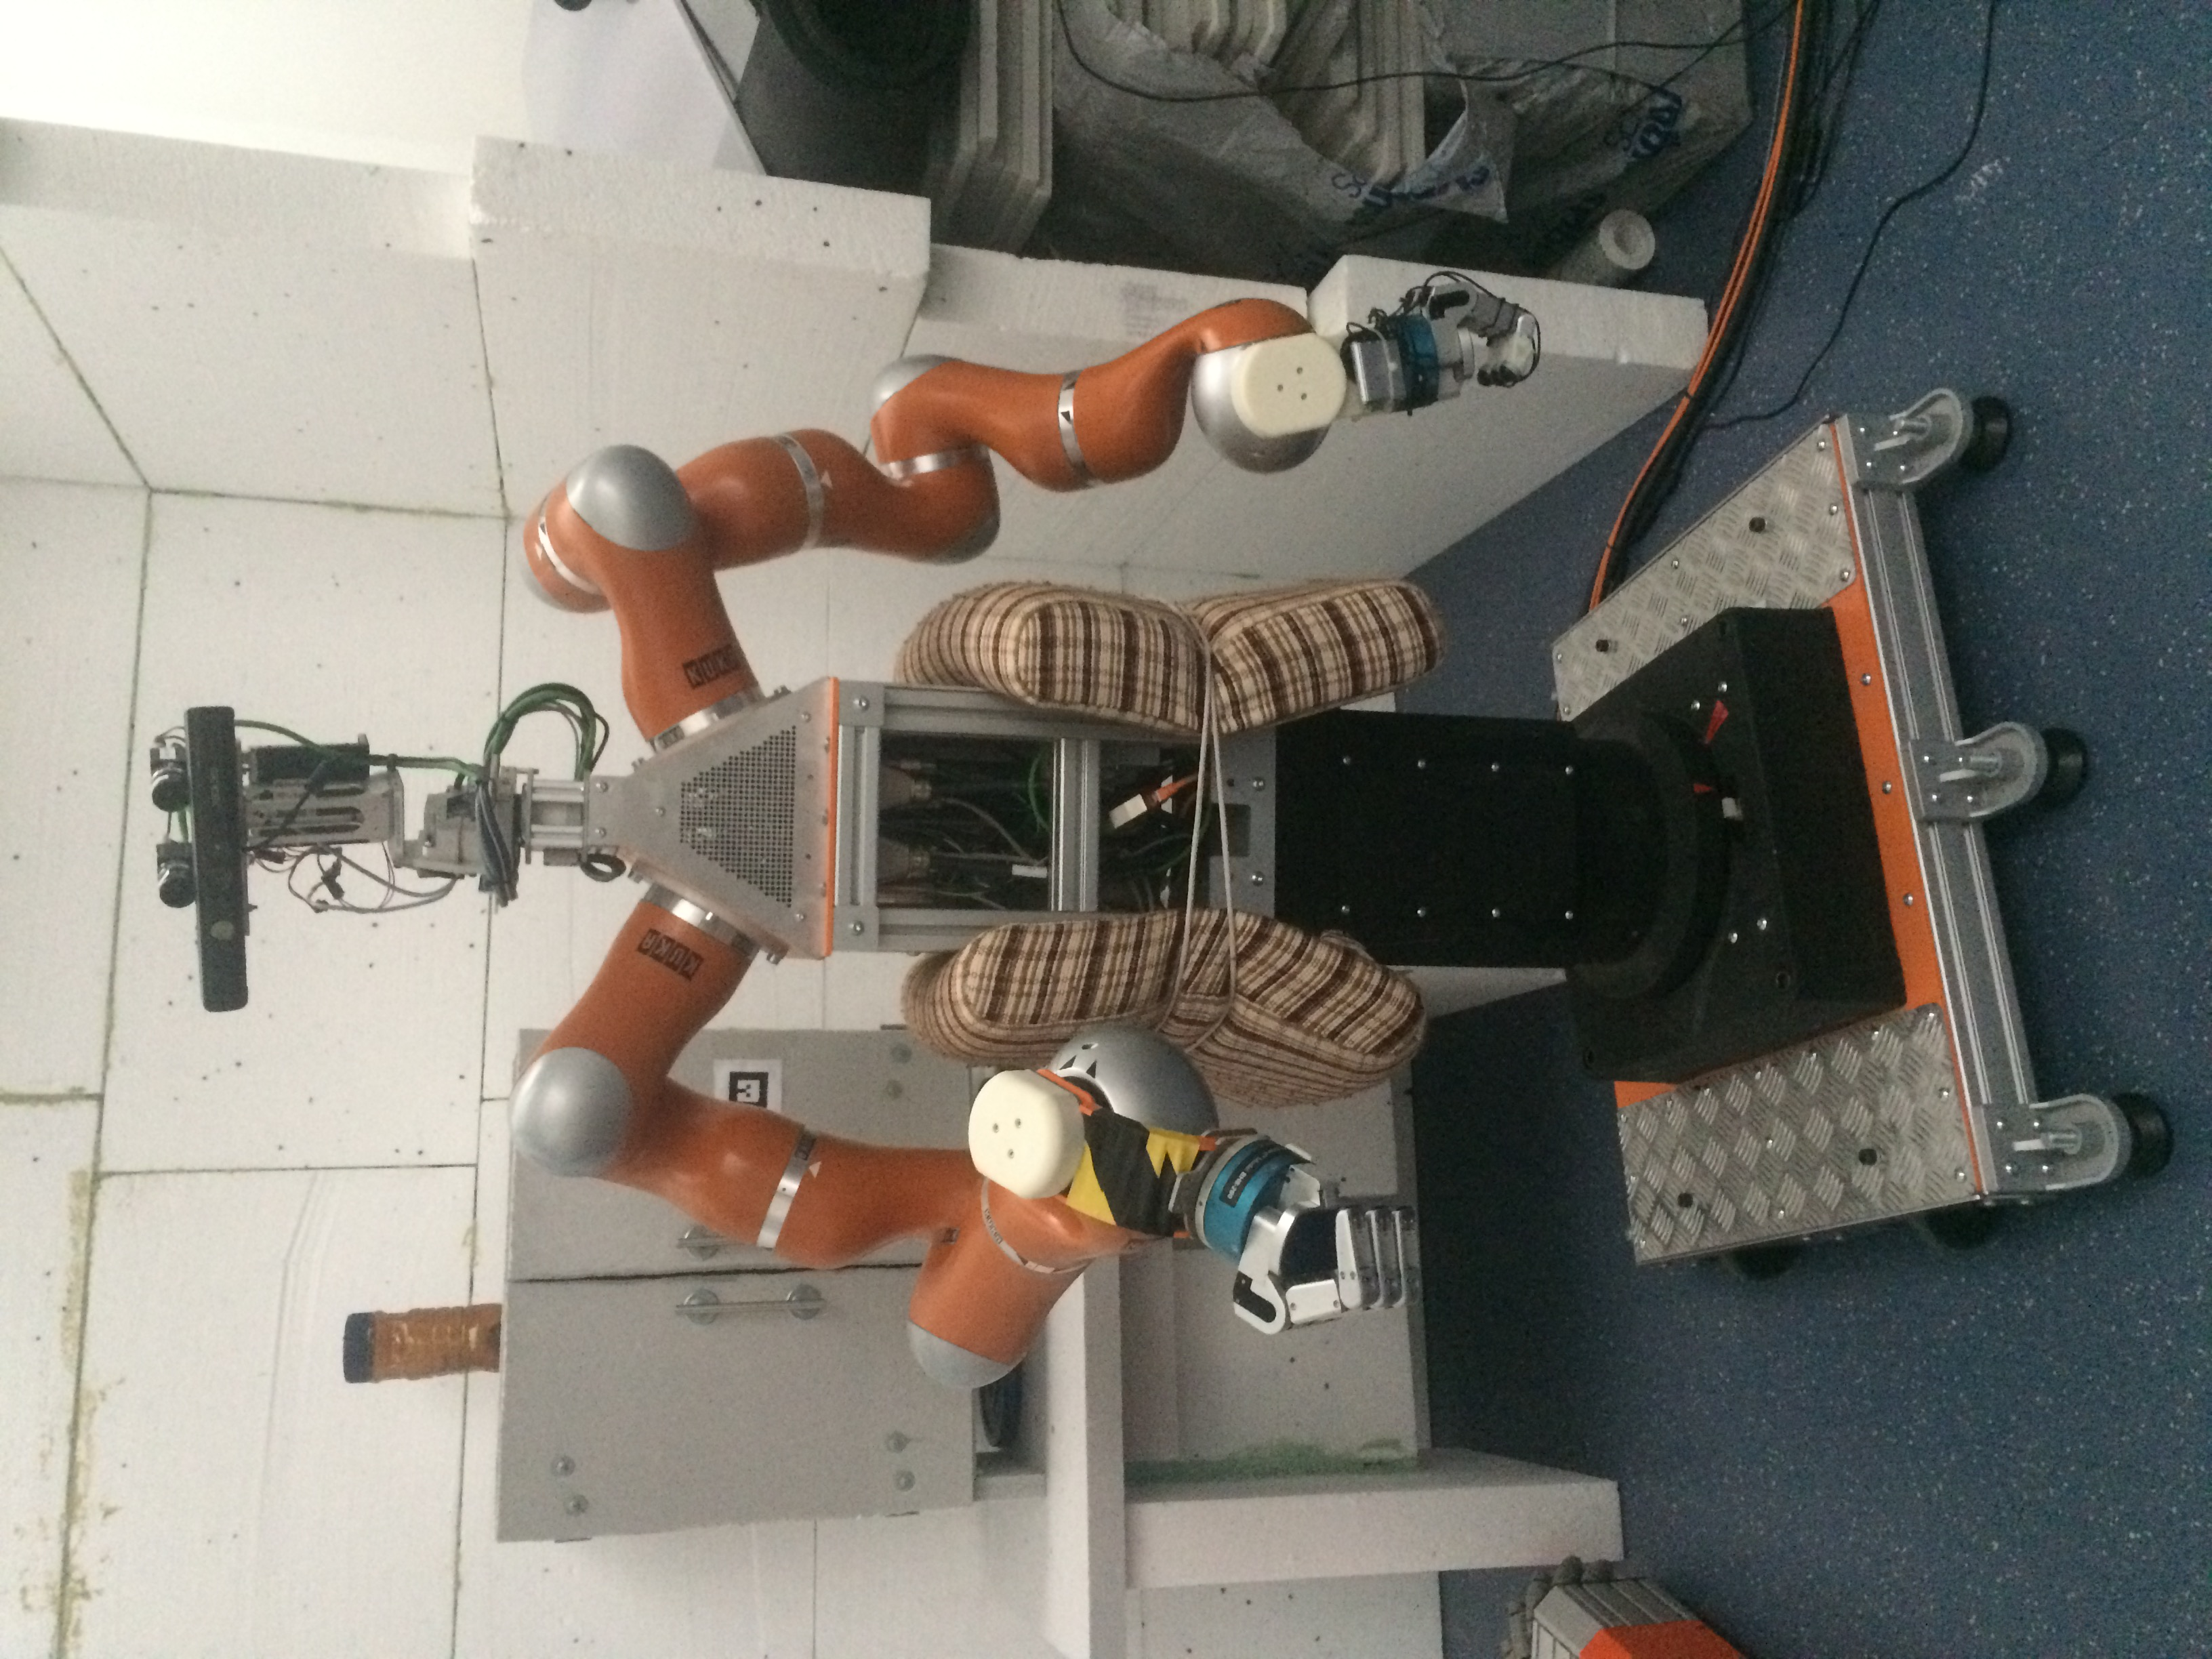
\includegraphics[scale=0.06, angle =-90]{velma1}
\end{figure}

\end{frame}

\begin{frame}{Robot usługowy Velma}
\begin{itemize}
\item Dwa manipulatory LWR (sterowanie impedancyjne)
\item Chwytaki Barretta (sztuczna skóra, czujniki siły)
\item Nadgarstkowe czujniki siły i momentu
\item Kinect
\item Stereopara
\item Baza jezdna z kołami Mecanum
\end{itemize}
\end{frame}
\begin{frame}{Oprogramowanie robota Velma}

Struktura komponentowa. Częstotliwość pętli sterowania to 500 Hz.

\begin{itemize}
	\item ROS
	\item Orocos
\end{itemize}

Symulator działania z modelem fizyki i symulacją czasu.


\begin{itemize}
	\item Gazebo
	\item Dart
\end{itemize}
\end{frame}

\section{Porównanie pracy magisterskiej z inżynierską}
\begin{frame}{Sterowanie niskopoziomowe robota Elektron}
Celem pracy było wytworzenie oprogramowania urządzeń robota takiego, że będzie możliwa praca zgodnie z reżimem czasu rzeczywistego. Praca pod kierownictwem dra inż. Tomasza Winiarskiego.
\begin{itemize}
	\item Robot mobilny Elektron z napędem różnicowym
	\item Napisanie oprogramowania mikrokontrolera robota
	\item STM32F107
	\item FreeRTOS
	\item RS-232
\end{itemize}
\end{frame}

\begin{frame}{Robot mobilny Elektron}

\begin{figure}[h]
	\centering
	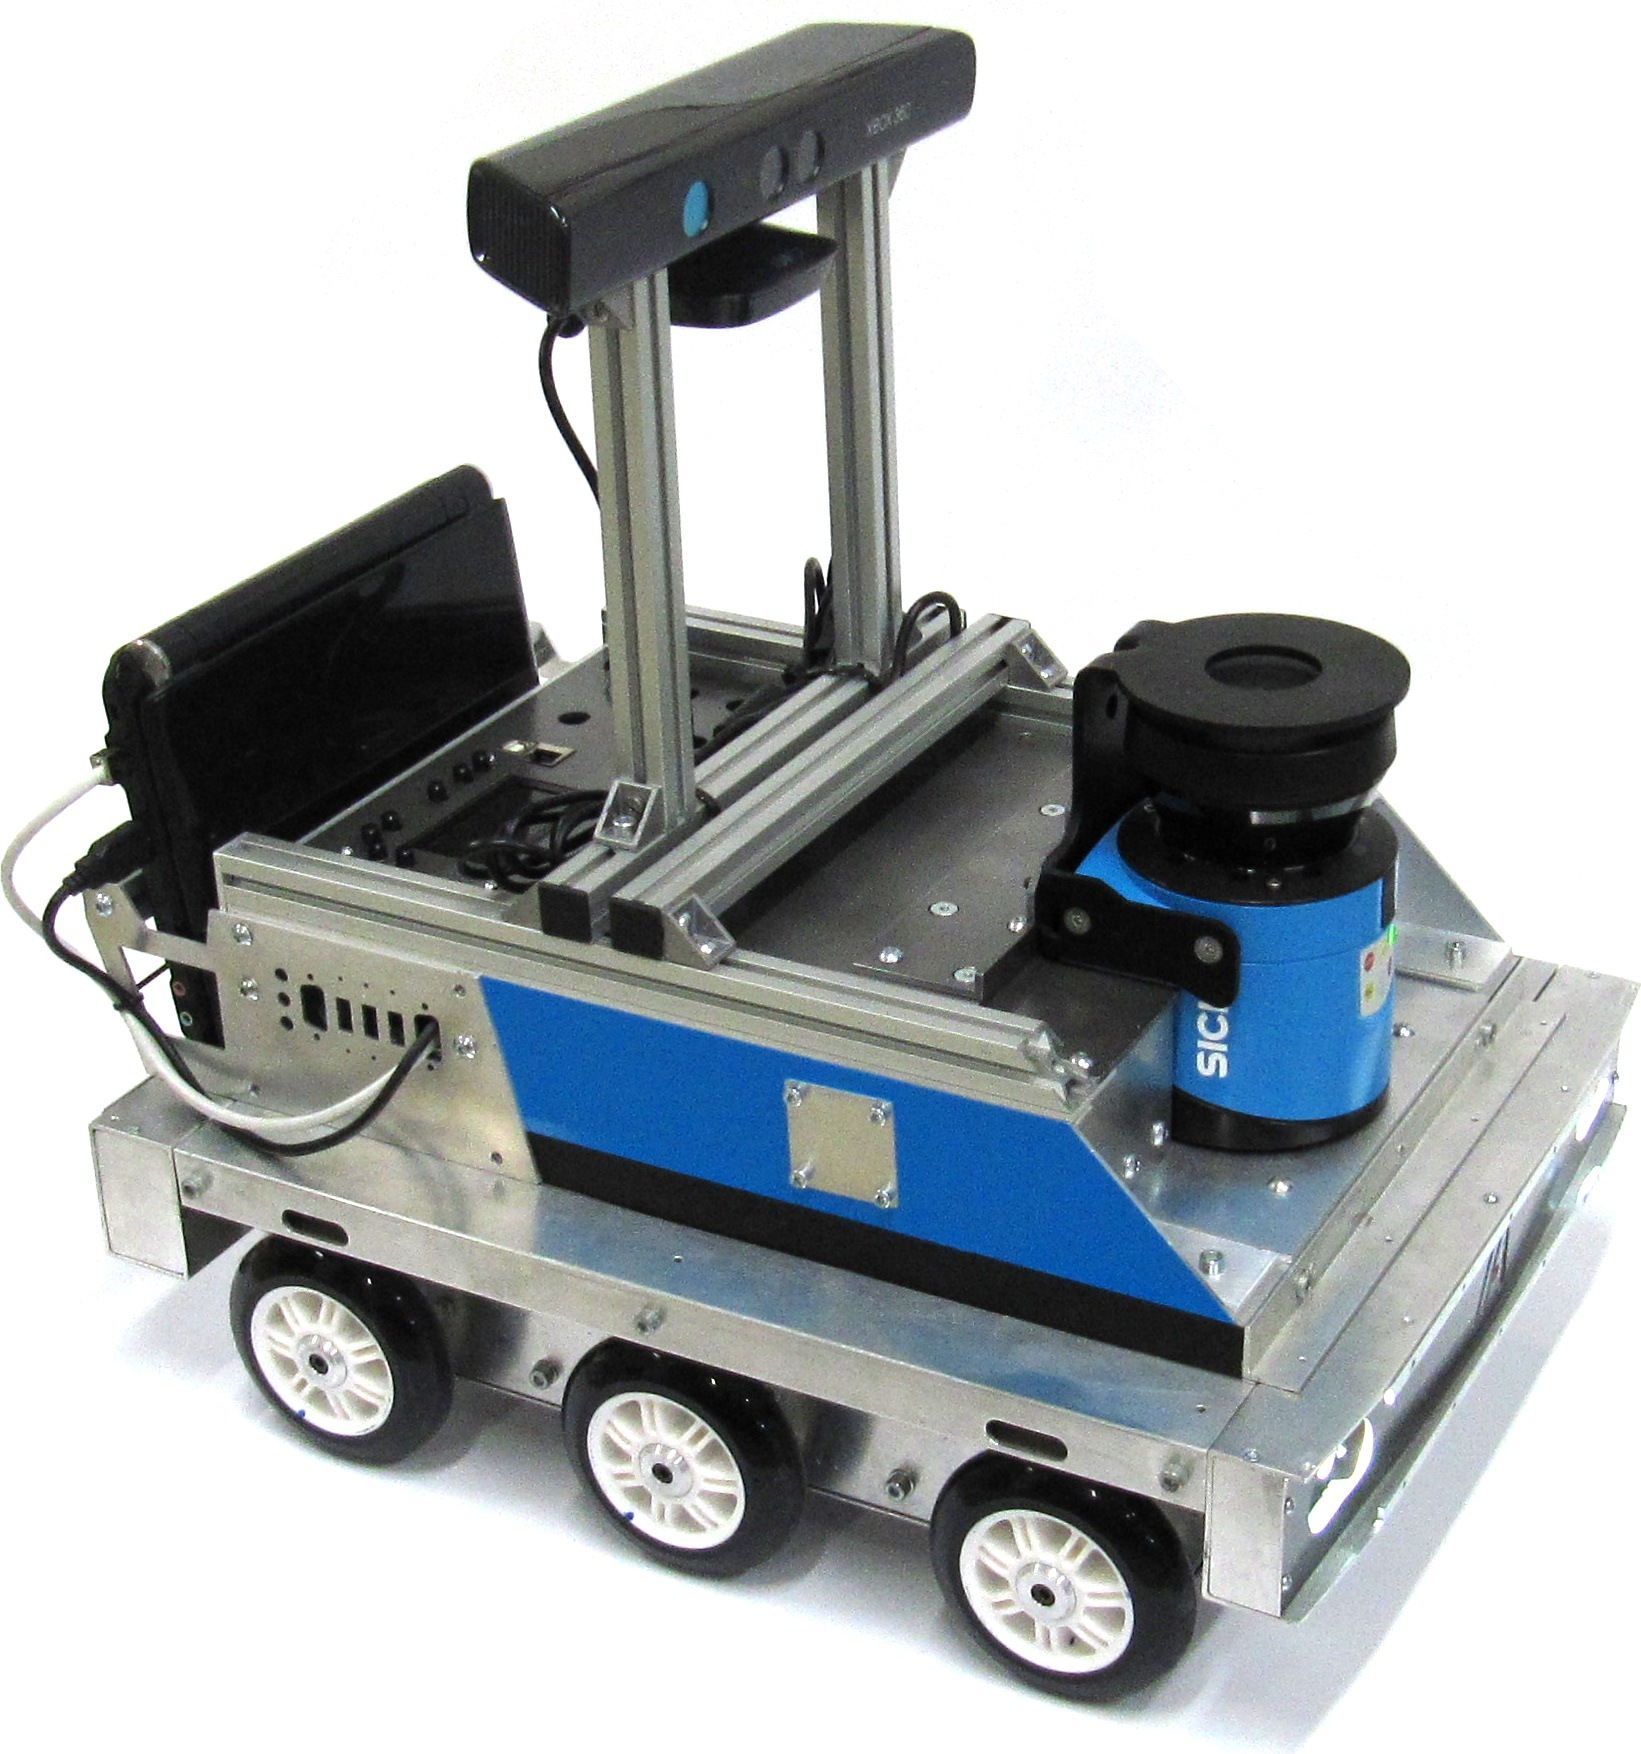
\includegraphics[scale=0.1]{elektron}
\end{figure}

\end{frame}

\begin{frame}{Podobieństwa}
\begin{itemize}
	\item Promotor
	\item Związek obu prac z robotyką
\end{itemize}
\end{frame}
\begin{frame}{Różnice}
Praca magisterska nie jest kontynuacją pracy inżynierskiej.
\begin{itemize}
	\item Cele prac nastawione są na innego typu rezultaty
	\item Różne platformy badawcze
	\item Praca inżynierska nastawiona na pracę ze sprzętem
	\item Praca magisterska nastawiona na odkrycie algorytmu
	\item Nieznany końcowy rezultat pracy magisterskiej
\end{itemize}
\end{frame}
%\begin{frame}[allowframebreaks]{Bibliografia}
%\bibliographystyle{plain}
%\bibliography{bibliography}
%\end{frame}
\section{Zakończenie}
\begin{frame}{Bibliografia}
Zdjęcia pochodzą ze strony \url{https://robotyka.ia.pw.edu.pl}
\end{frame}
\begin{frame}{Dziękuję za uwagę}
\begin{figure}[h]
	\centering
	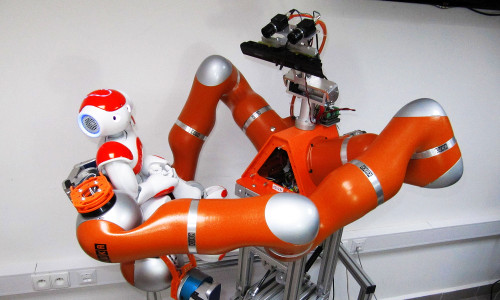
\includegraphics[scale=1.4]{velma3}
\end{figure}
\end{frame}
\end{document}